\section*{Lab 4 -- Parallel Processing and SIMD Evaluation}
\addcontentsline{toc}{section}{Lab 4 -- Parallel Processing and SIMD Evaluation}

This laboratory activity addresses \textbf{Lab~4 -- Parallel Processing} and focuses on the
analysis of task-level and data-level parallelism on the dual-core ARM Cortex-A9
architecture of the Zybo~Z7 board. The experiment is conducted in a bare-metal
environment and aims at evaluating both the benefits and limitations of parallel
execution and SIMD auto-vectorization on a shared-memory embedded platform.

The core objective of the lab is the design and evaluation of a shared-memory
parallel application in which \textbf{Core~0 (Master)} and \textbf{Core~1 (Worker)}
cooperate to compute a vector addition. Two input vectors $A$ and $B$ are allocated
in shared DDR memory, and the resulting vector $C$ is computed as
\[
C[i] = A[i] + B[i].
\]
The computational workload is evenly partitioned between the two cores, with
Core~0 processing the first half of the vector and Core~1 processing the second half.
Inter-core coordination is achieved through a minimal synchronization mechanism
based on shared memory flags (\texttt{start}, \texttt{done0}, \texttt{done1}), without
any operating system support.

Execution time is measured using the ARM Cortex-A9 Global Timer, allowing a
quantitative comparison between serial and parallel implementations. In addition,
the impact of data-level parallelism is investigated by enabling compiler
auto-vectorization through ARM NEON SIMD instructions. Overall, the laboratory
provides insight into low-level multi-core programming, explicit workload
partitioning, shared-memory communication, synchronization, and performance
evaluation on embedded systems.

\subsection*{System Debugger Configuration}
\addcontentsline{toc}{subsection}{System Debugger Configuration}

To ensure correct and deterministic execution, a \textit{System Debugger} run
configuration was created in the Xilinx SDK environment. Before launching the
application, the system is fully reset and the FPGA fabric (PL) is reprogrammed.
The Processing System (PS) is initialized through the execution of
\texttt{ps7\_init}, followed by \texttt{ps7\_post\_config}, which enables the
level shifters between PL and PS.

The two application binaries are explicitly assigned to the corresponding
processors, with \texttt{master.elf} mapped to Processor~0 and \texttt{worker.elf}
mapped to Processor~1. Automatic processor reset and stopping at program entry are
disabled to allow both cores to start execution simultaneously. This configuration
is essential to obtain reliable timing measurements and correct inter-core
synchronization.

\subsection*{Linker Script Modification}
\addcontentsline{toc}{subsection}{Linker Script Modification}

In order to support a shared-memory dual-core execution model, the linker script
(\texttt{lscript.ld}) was explicitly modified for both applications. The memory
layout was carefully configured to ensure that executable code, global and static
data, stack, and heap are all placed in DDR memory regions accessible by both
processors, while avoiding any overlap with the shared communication area.

The shared DDR region used for inter-core communication is excluded from all
linker-managed sections, preventing accidental overwriting by either core.
This modification is a critical requirement for correctness and determinism in
bare-metal multi-core systems and follows the memory layout prescribed in the
laboratory instructions.
\begin{figure}[H]
    \centering
    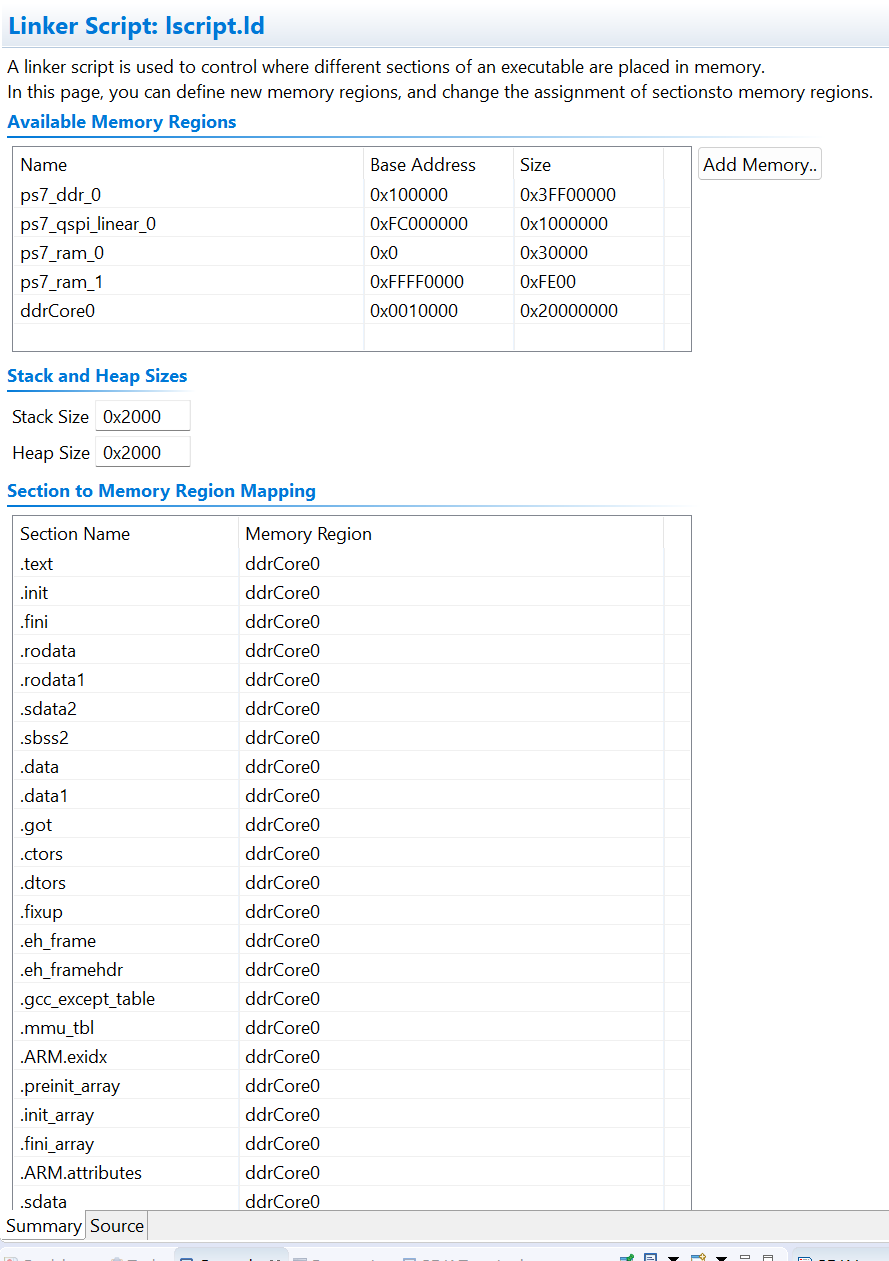
\includegraphics[width=0.95\linewidth]{images/master_lscript}
    \caption{Modified linker script for the Master application (Core~0).
    All sections are placed in DDR while avoiding overlap with the shared-memory region.}
    \label{fig:lab4_master_lscript}
\end{figure}

\begin{figure}[H]
    \centering
    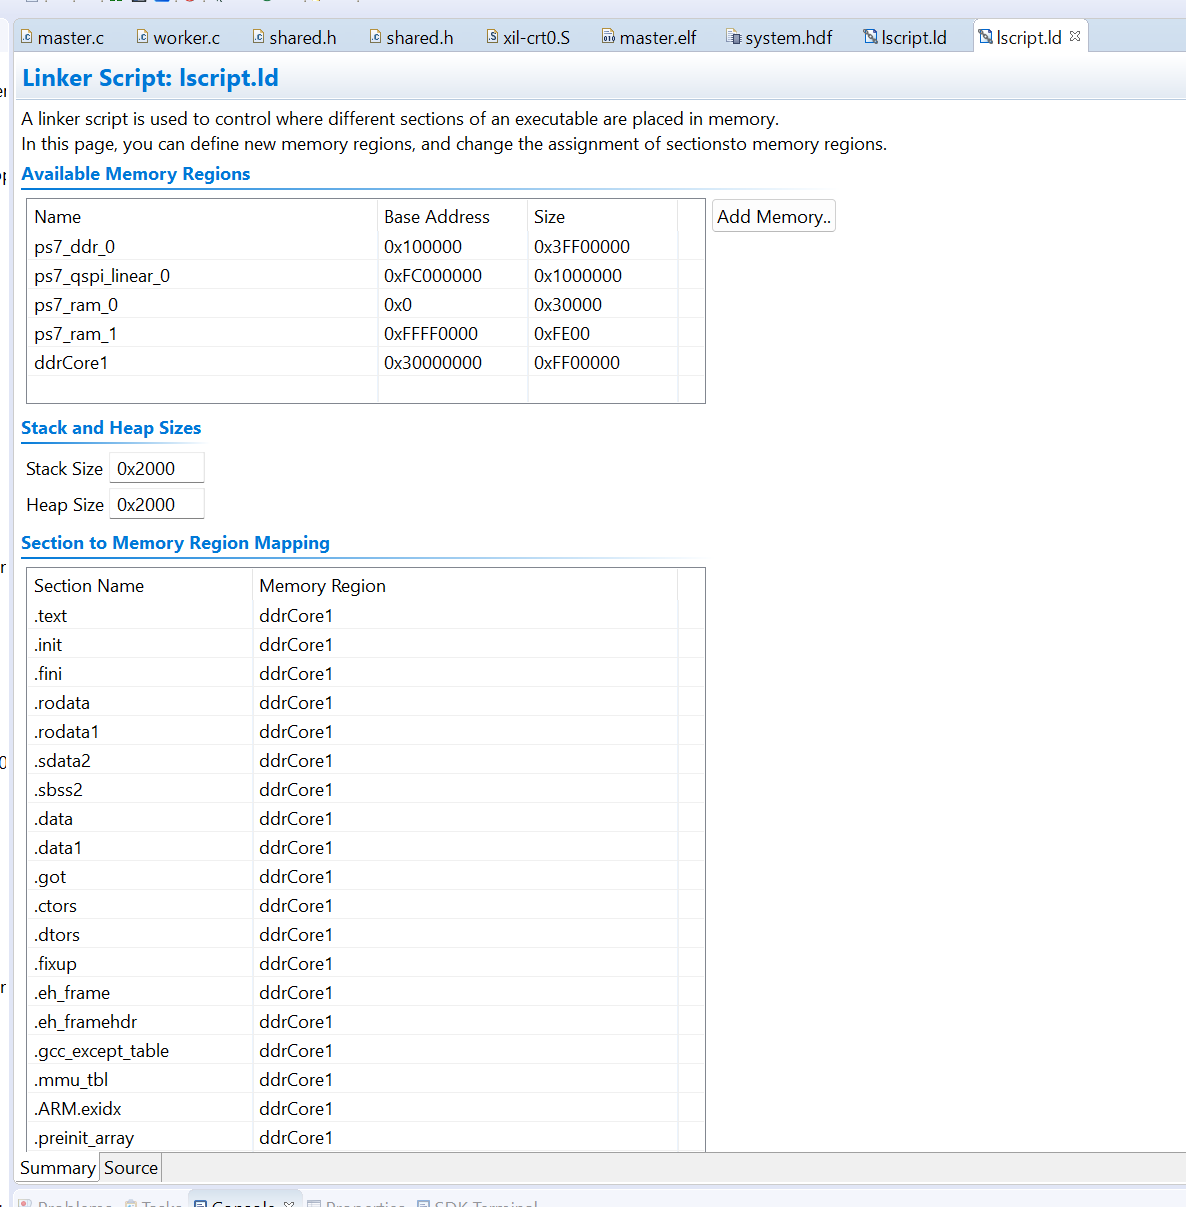
\includegraphics[width=0.95\linewidth]{images/worker_lscript}
    \caption{Modified linker script for the Worker application (Core~1).
    The shared DDR region is excluded from all linker-managed sections.}
    \label{fig:lab4_worker_lscript}
\end{figure}


\subsection*{Serial Baseline Integration}
\addcontentsline{toc}{subsection}{Serial Baseline Integration}

To provide a meaningful reference for performance evaluation, a serial baseline
implementation of the vector addition was integrated into the master application.
The function executes entirely on Core~0 and serves as a baseline for comparison
with the parallel implementation. The use of the \texttt{restrict} qualifier
enables the compiler to apply aggressive optimizations and auto-vectorization,
facilitating the evaluation of SIMD effectiveness independently of task-level
parallelism.

\subsection*{Compilation Settings}
\addcontentsline{toc}{subsection}{Compilation Settings}

Both the \texttt{master} and \texttt{worker} applications were compiled using
aggressive optimization settings, explicitly enabling ARM NEON support and
compiler auto-vectorization. The selected compiler and linker flags allow the
generation of SIMD instructions and provide diagnostic feedback on vectorization
decisions. This configuration ensures that both task-level parallelism and
instruction-level parallelism are exploited to the maximum extent allowed by the
architecture and memory subsystem.
\begin{figure}[H]
    \centering
    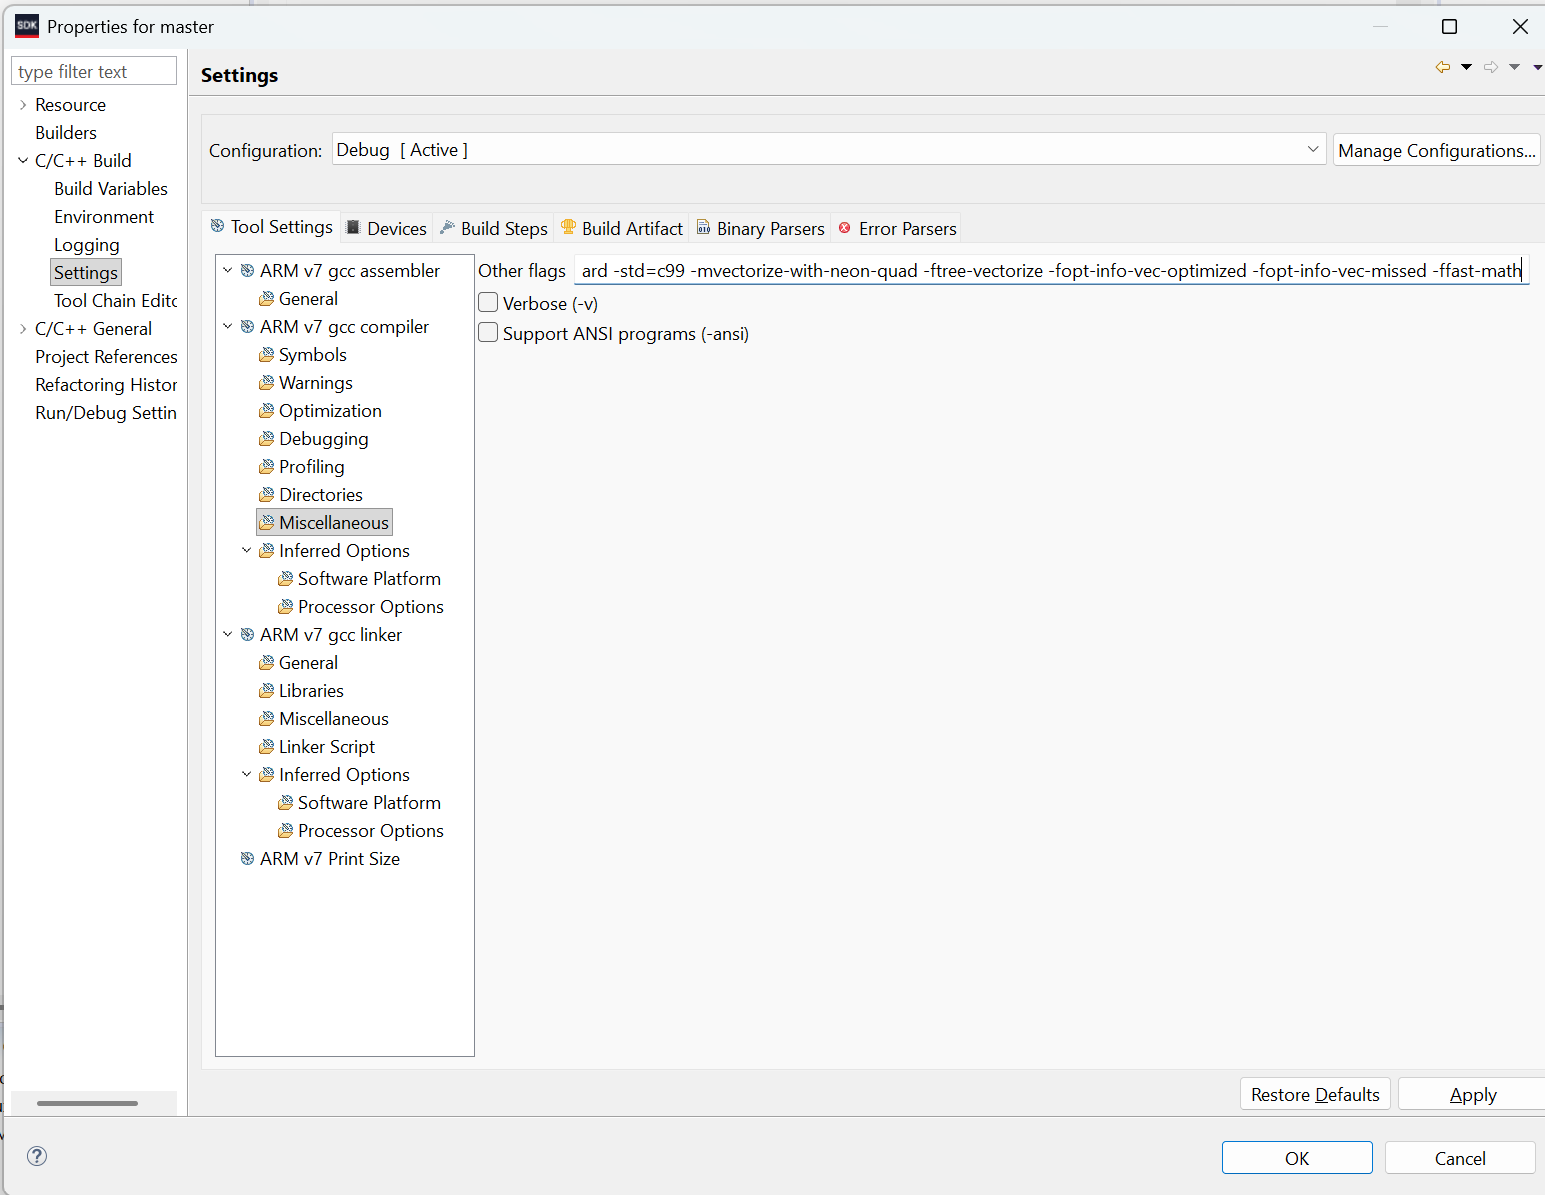
\includegraphics[width=0.9\linewidth]{images/master_compiler}
    \caption{Compiler optimization and auto-vectorization flags used for the Master application.}
    \label{fig:lab4_master_compiler}
\end{figure}

\begin{figure}[H]
    \centering
    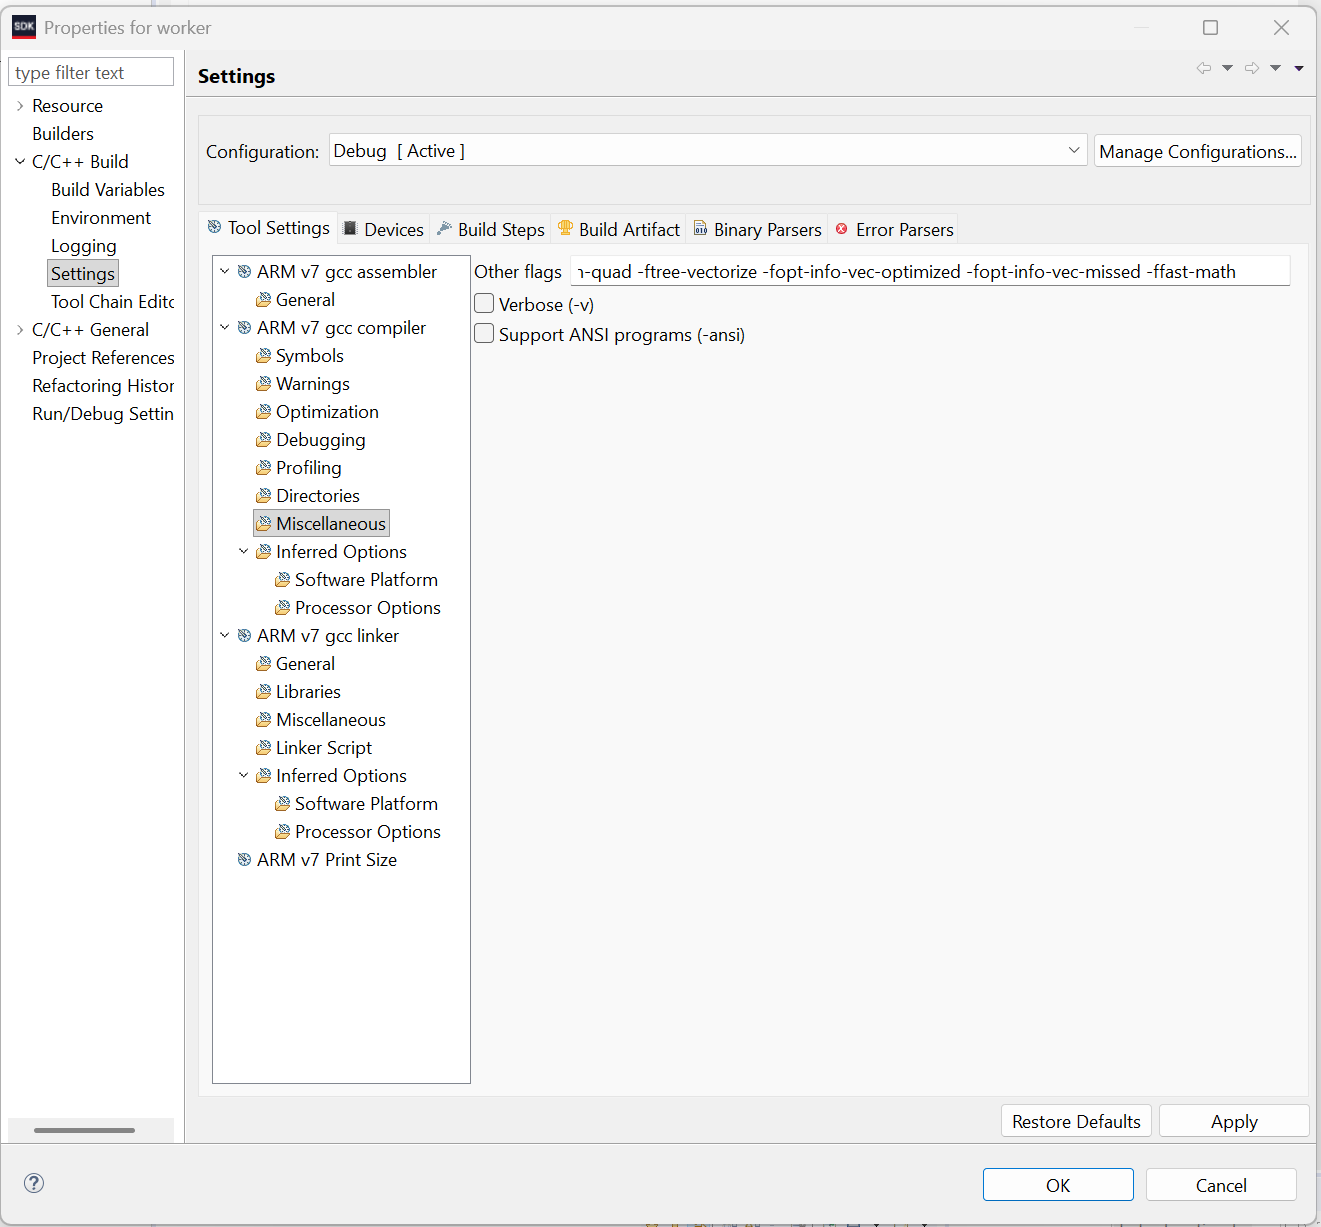
\includegraphics[width=0.9\linewidth]{images/worker_compiler}
    \caption{Compiler optimization and auto-vectorization flags used for the Worker application.}
    \label{fig:lab4_worker_compiler}
\end{figure}

\begin{figure}[H]
    \centering
    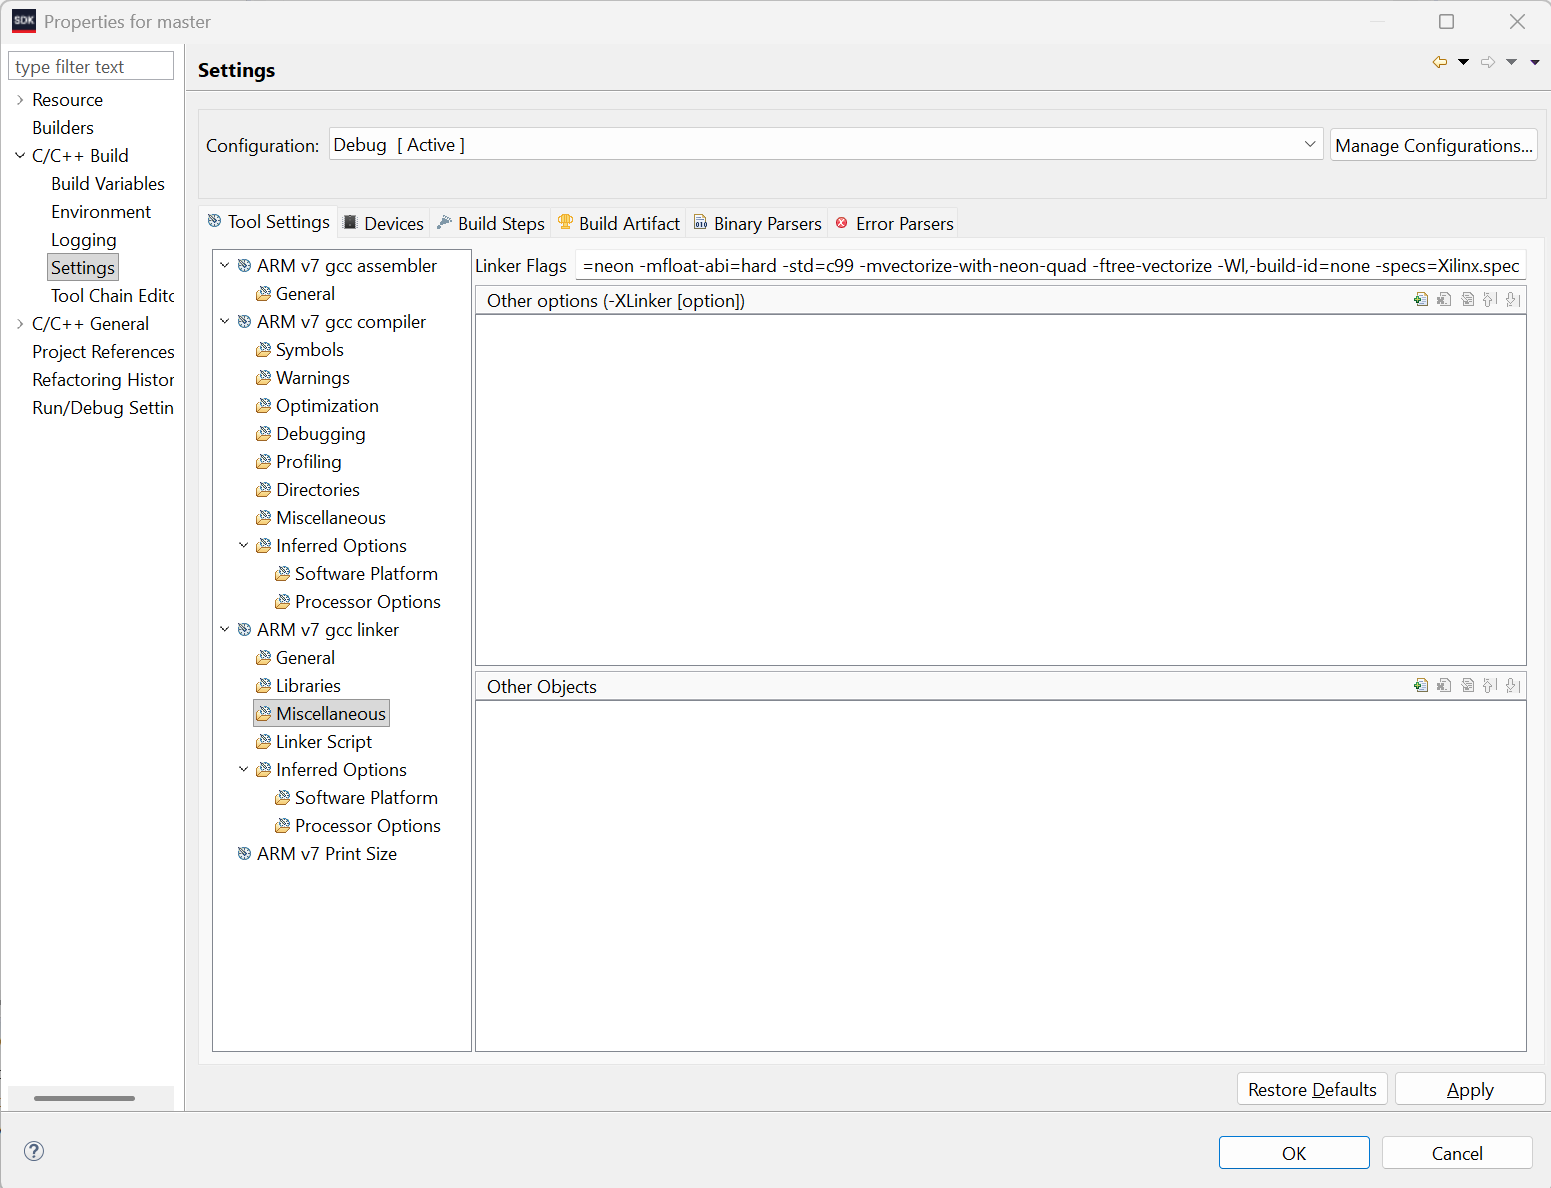
\includegraphics[width=0.9\linewidth]{images/master_linker}
    \caption{Linker configuration for the Master application.}
    \label{fig:lab4_master_linker}
\end{figure}

\begin{figure}[H]
    \centering
    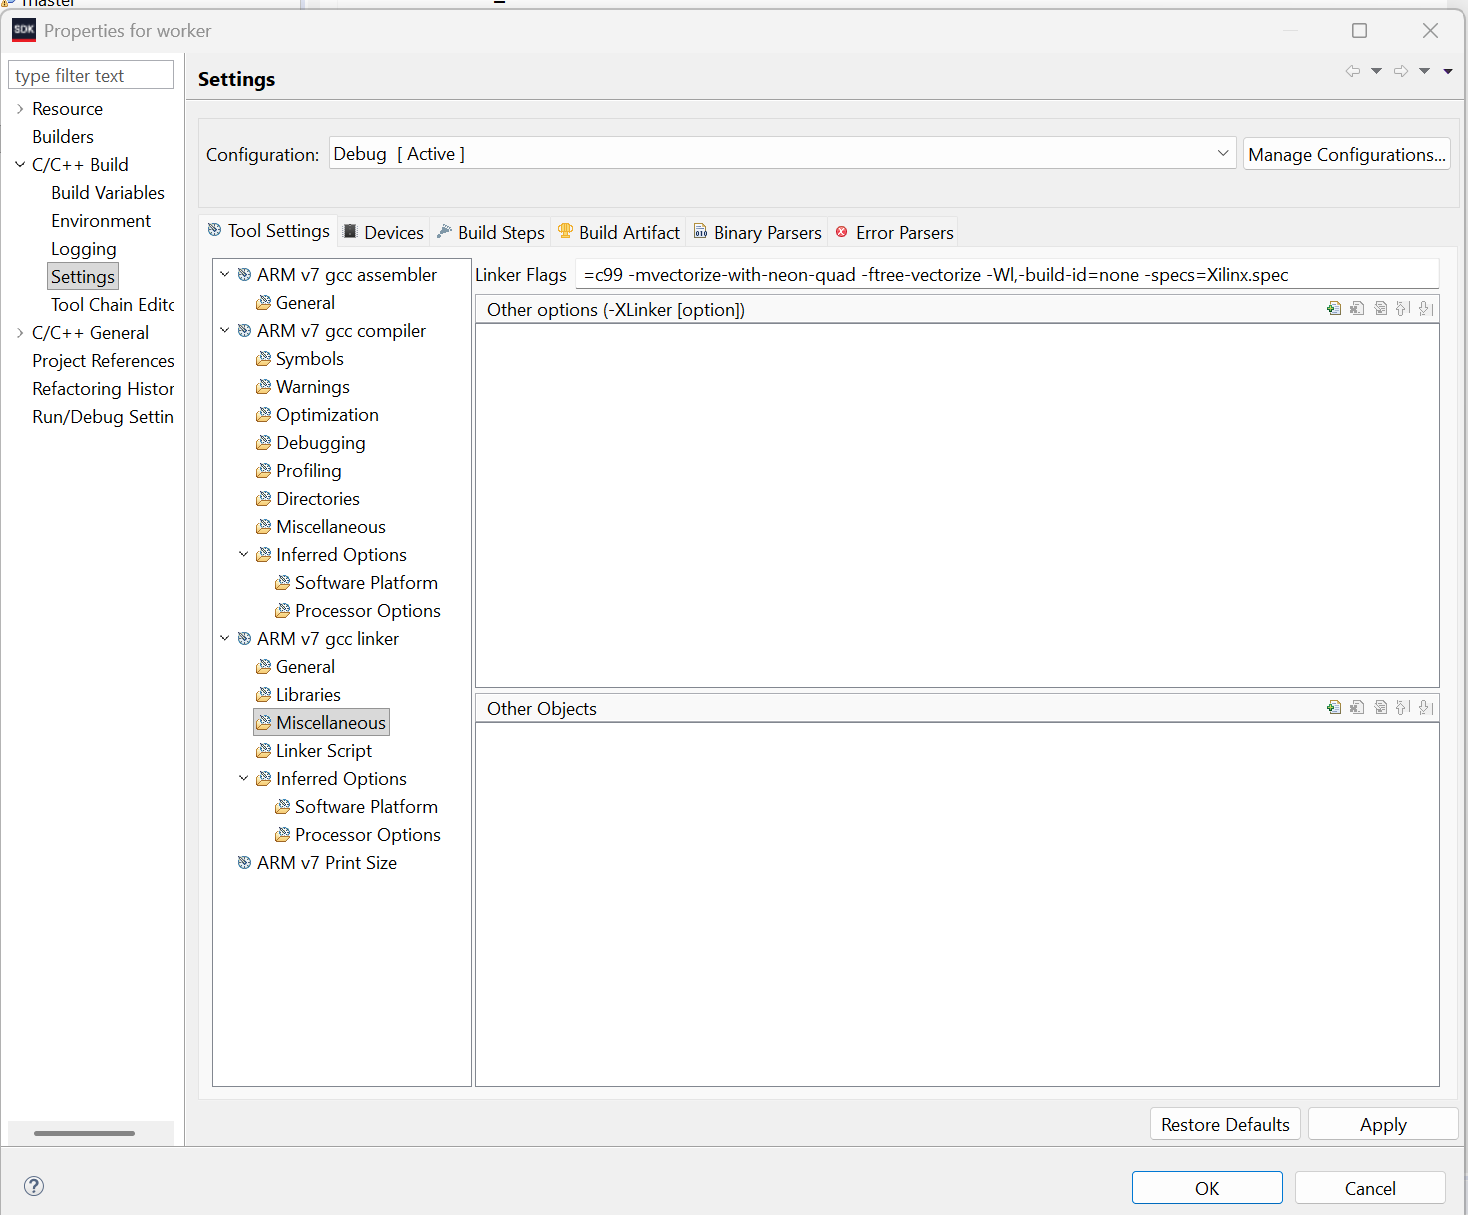
\includegraphics[width=0.9\linewidth]{images/worker_linker}
    \caption{Linker configuration for the Worker application.}
    \label{fig:lab4_worker_linker}
\end{figure}

\subsection*{Execution Time Measurements}
\addcontentsline{toc}{subsection}{Execution Time Measurements}

Execution time measurements were performed using the ARM Cortex-A9 Global Timer
and expressed in CPU cycles. Experiments were conducted for multiple array sizes
(\texttt{ARRAY\_SIZE = 10}, \texttt{100}, \texttt{1000}, and \texttt{10000}) to assess
the scalability of the proposed parallel approach.

The obtained results, summarized in Table~\ref{tab:lab4_timing_results} and supported
by the UART outputs reported in Figures~\ref{fig:lab4_10}--\ref{fig:lab4_10000},
show that parallel execution does not provide a significant speedup with respect
to the serial baseline. For all tested configurations, the parallel implementation
exhibits execution times comparable to, or higher than, the serial version, resulting
in a speedup consistently lower than one.

From an architectural perspective, this behavior is expected. The vector addition
kernel is strongly memory-bound, and both cores concurrently access the same shared
DDR memory. As a consequence, memory bandwidth contention dominates execution time,
limiting the benefits of task-level parallelism despite the even workload partitioning
and the minimal synchronization overhead.



\begin{figure}[H]
    \centering
    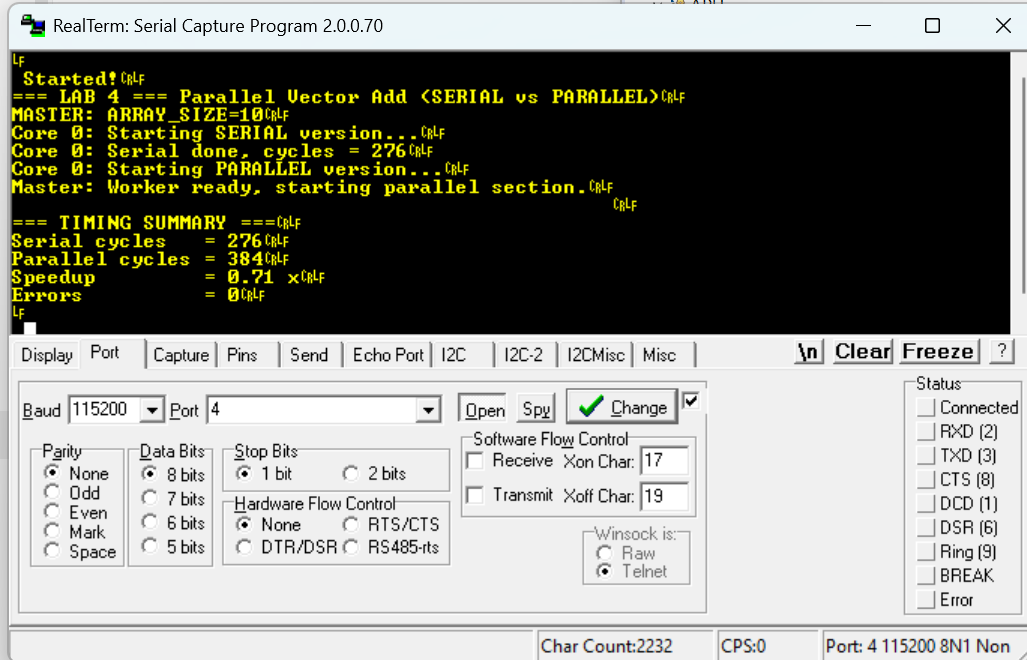
\includegraphics[width=0.9\linewidth]{images/lab4_10}
    \caption{UART output for the parallel vector addition with \texttt{ARRAY\_SIZE = 10}.}
    \label{fig:lab4_10}
\end{figure}


\begin{figure}[H]
    \centering
    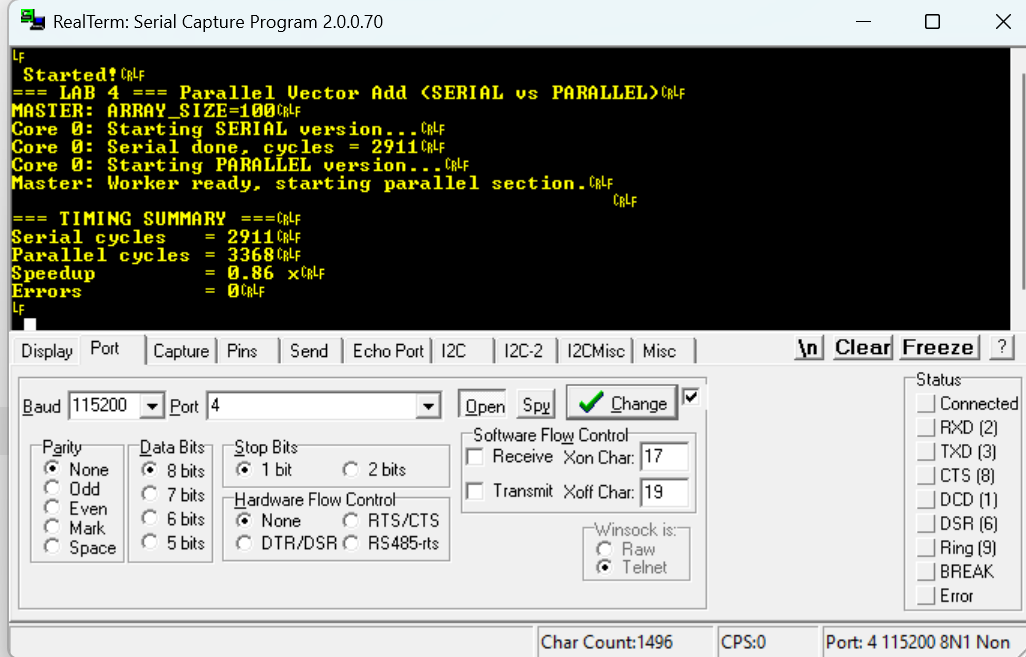
\includegraphics[width=0.9\linewidth]{images/lab4_100}
    \caption{UART output for the parallel vector addition with \texttt{ARRAY\_SIZE = 100}.}
    \label{fig:lab4_100}
\end{figure}

\begin{figure}[H]
    \centering
    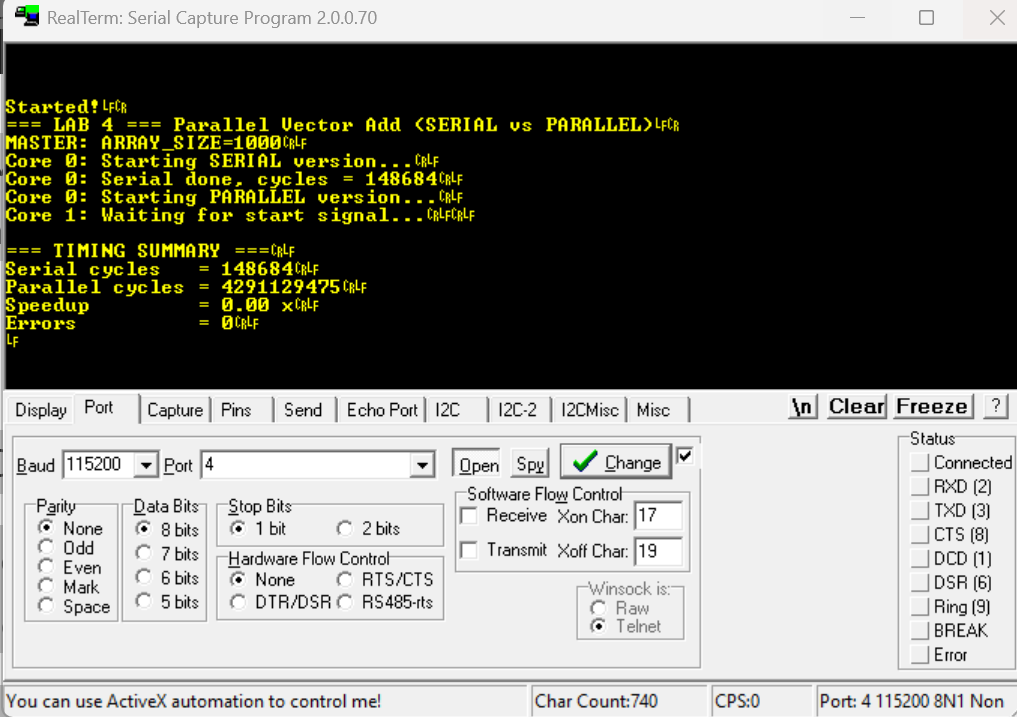
\includegraphics[width=0.9\linewidth]{images/lab4_1000}
    \caption{UART output for the parallel vector addition with \texttt{ARRAY\_SIZE = 1000}.}
    \label{fig:lab4_1000}
\end{figure}

\begin{figure}[H]
    \centering
    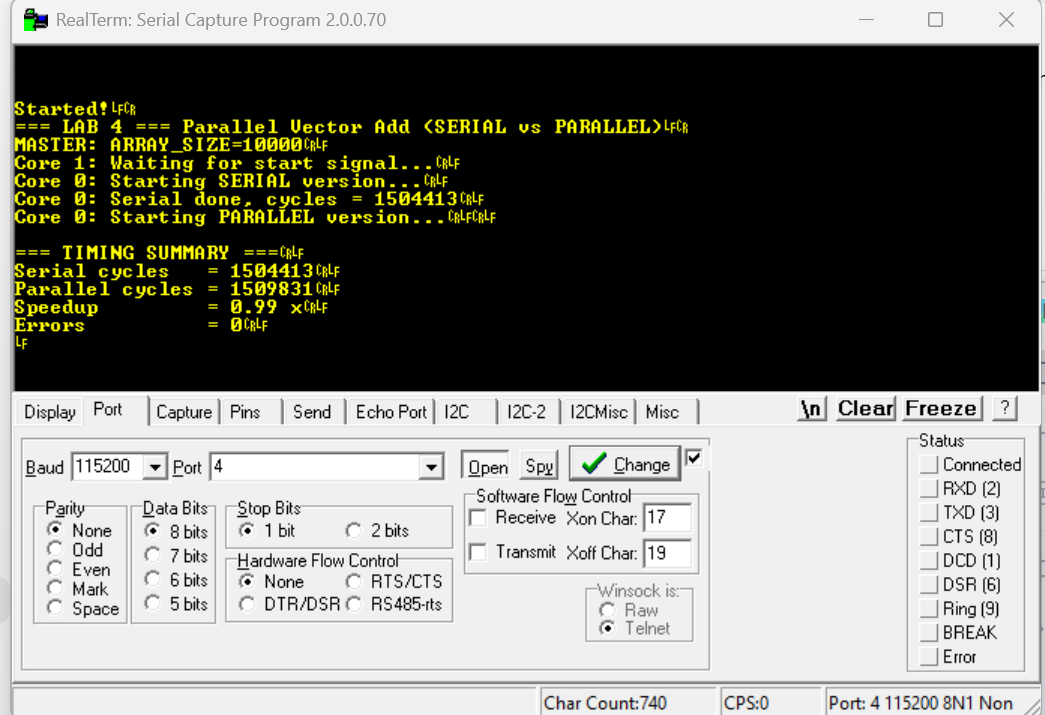
\includegraphics[width=0.9\linewidth]{images/lab4_10000}
    \caption{UART output for the parallel vector addition with \texttt{ARRAY\_SIZE = 10000}.}
    \label{fig:lab4_10000}
\end{figure}


\begin{table}[H]
\centering
\caption{Execution time comparison between serial and parallel implementations
for different array sizes (Lab 4).}
\label{tab:lab4_timing_results}
\renewcommand{\arraystretch}{1.2}
\begin{tabular}{|c|r|r|c|}
\hline
\textbf{ARRAY\_SIZE} &
\textbf{Serial cycles} &
\textbf{Parallel cycles} &
\textbf{Speedup} \\
\hline
10     & 276     & 384     & 0.71$\times$ \\
100    & 2911    & 3368    & 0.86$\times$ \\
1000   & 27644   & 32803   & 0.84$\times$ \\
10000  & 325098  & 591334  & 0.54$\times$ \\
\hline
\end{tabular}
\end{table}


\subsection*{Discussion in Light of Amdahl's Law}
\addcontentsline{toc}{subsection}{Discussion in Light of Amdahl's Law}

The experimental results obtained in Lab~4 can be formally interpreted using
\textit{Amdahl's Law}, which provides an upper bound on the achievable speedup of a
parallel program as a function of the fraction of code that can be parallelized.
According to Amdahl's formulation, the theoretical speedup $S(N)$ obtained using
$N$ processing units is given by:
\[
S(N) = \frac{1}{(1 - P) + \frac{P}{N}},
\]
where $P$ represents the fraction of the execution time that can be parallelized,
and $(1 - P)$ corresponds to the inherently serial portion of the workload.

In the implemented vector addition kernel, the computational loop is fully
parallelizable in principle ($P \approx 1$). However, the experimental measurements
show speedup values consistently lower than one (Table~\ref{tab:lab4_timing_results}),
with measured speedups ranging from approximately $0.71\times$ for
\texttt{ARRAY\_SIZE = 10} to $0.54\times$ for \texttt{ARRAY\_SIZE = 10000}.
This indicates that the effective parallel fraction $P$ is significantly reduced
by architectural constraints.

In particular, although the arithmetic operations are parallelized across the two
cores, both processors concurrently access the same shared DDR memory. As a result,
memory access latency and bandwidth contention dominate execution time, effectively
introducing a large serial component that limits scalability. In this context,
the memory subsystem behaves as the true bottleneck of the system, reducing the
benefits of task-level parallelism even when synchronization overhead is minimal.

Therefore, the observed lack of speedup is not due to inefficient parallelization,
but is a direct consequence of Amdahl's Law applied to a memory-bound workload on a
shared-memory embedded architecture. This experimental evidence highlights the
importance of considering memory hierarchy and bandwidth constraints when designing
parallel applications for embedded multi-core systems.


\subsection*{Assembly Inspection and SIMD Verification}
\addcontentsline{toc}{subsection}{Assembly Inspection and SIMD Verification}

To assess the effectiveness of data-level parallelism, the compiled
\texttt{master.elf} binary was inspected using the SDK disassembly view. The
analysis confirms that the serial baseline loop was successfully auto-vectorized
by the compiler.

The presence of ARM NEON instructions, such as vector loads
(\texttt{vld1.32}), vector additions (\texttt{vadd.i32}), and vector stores
(\texttt{vst1.32}), demonstrates that instruction-level parallelism is effectively
exploited. This confirms that the lack of performance improvement in the parallel
version is not due to suboptimal code generation, but rather to fundamental memory
system limitations.
\begin{figure}[H]
    \centering
    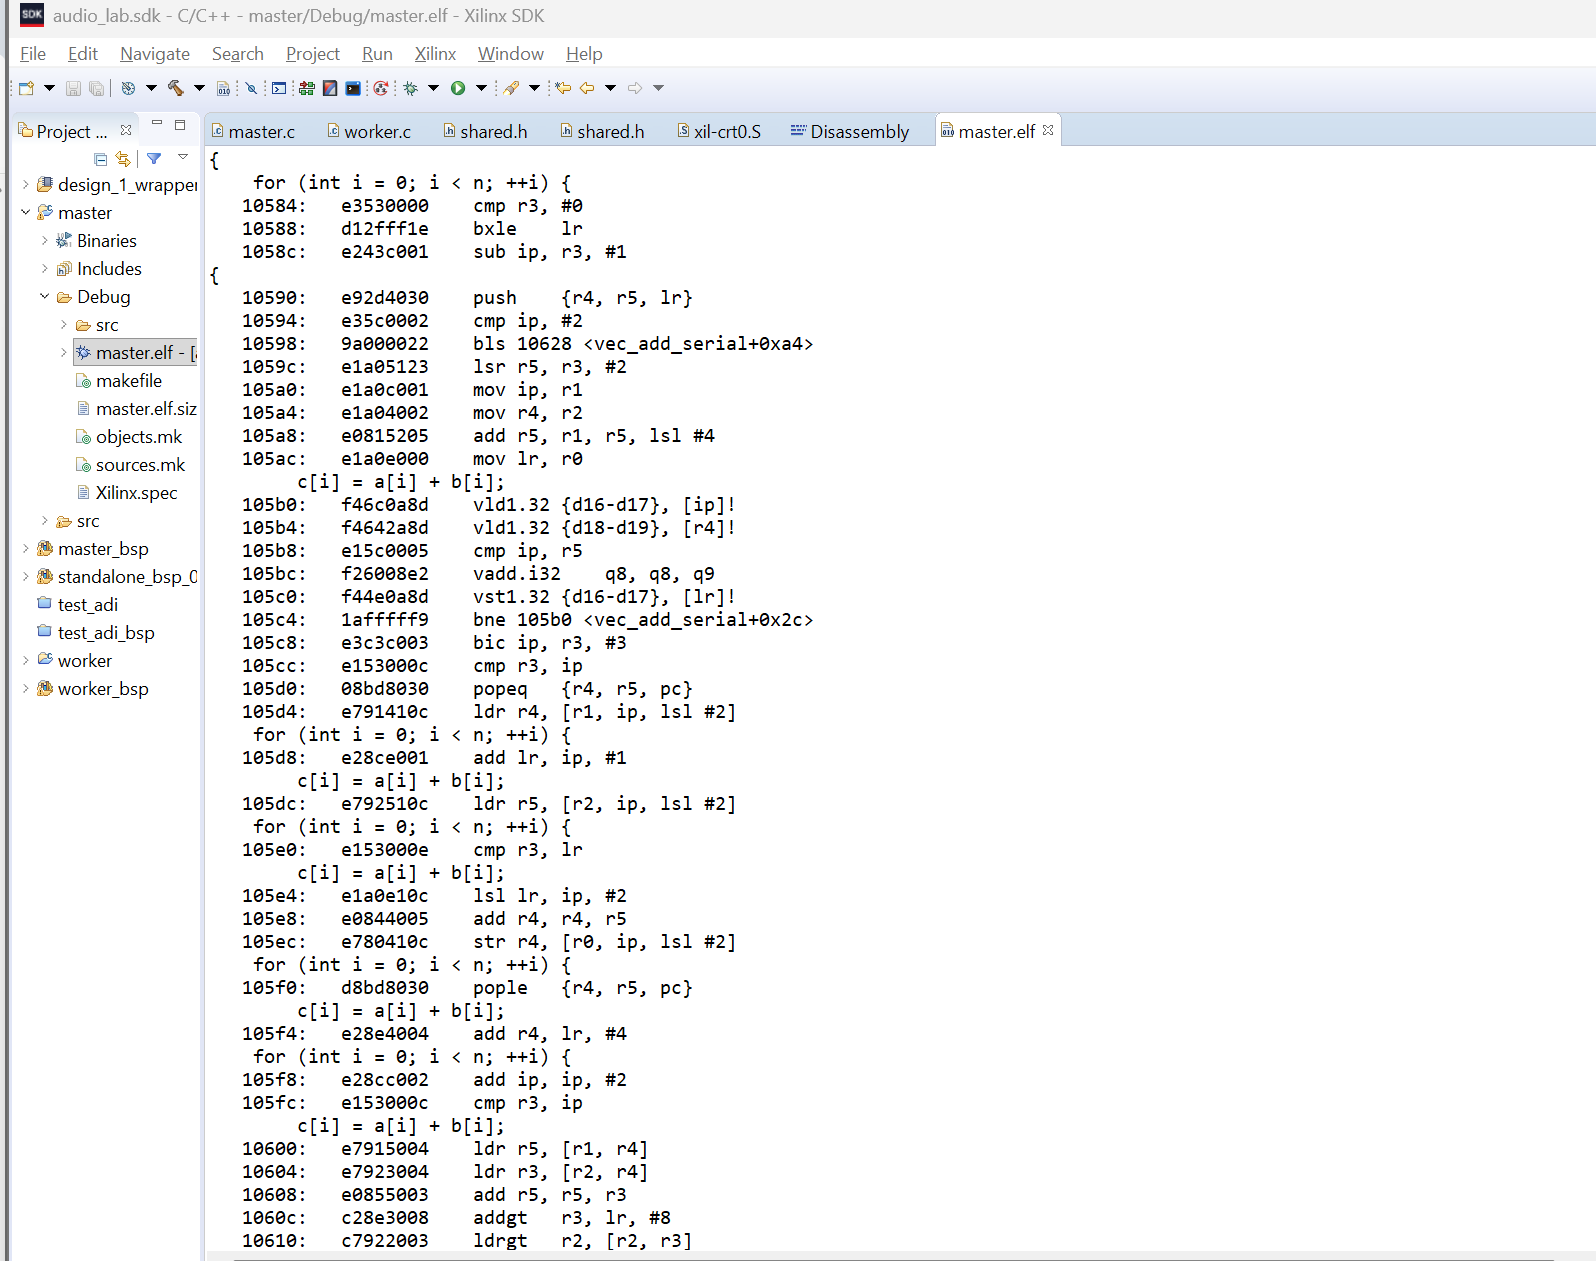
\includegraphics[width=0.95\linewidth]{images/master_elf}
    \caption{Disassembly of the serial baseline showing ARM NEON SIMD instructions
    (\texttt{vld1.32}, \texttt{vadd.i32}, \texttt{vst1.32}).}
    \label{fig:lab4_neon}
\end{figure}
\begin{figure}[H]
    \centering
    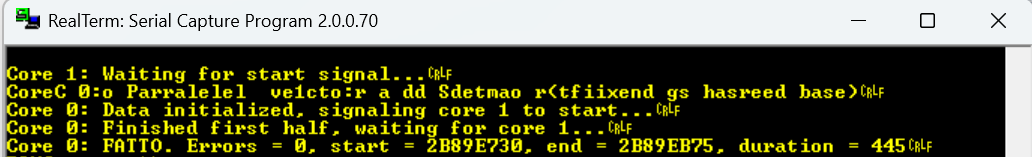
\includegraphics[width=0.9\linewidth]{images/lab4output}
    \caption{UART output showing correct parallel execution on both cores (Master and Worker).}
    \label{fig:lab4_output}
\end{figure}

\subsection*{Results Summary}
\addcontentsline{toc}{subsection}{Lab 4 -- Results Summary}

Execution time measurements were performed using the ARM Cortex-A9 Global Timer
to evaluate the impact of parallel execution and SIMD auto-vectorization on a
vector addition workload. The following array sizes were considered:
\texttt{ARRAY\_SIZE = 10}, \texttt{100},\texttt{1000}, and \texttt{10000}.

For all tested configurations, the parallel implementation running on two cores
does not provide a significant execution-time improvement compared to the serial
baseline. In some cases, the parallel version exhibits similar or slightly higher
execution times. This behavior is consistent across all array sizes.

The limited speedup is mainly due to the memory-bound nature of the workload.
Both cores concurrently access the same shared DDR memory, resulting in bandwidth
contention that dominates execution time and limits the benefits of task-level
parallelism.

Assembly inspection confirms that the serial baseline is successfully
auto-vectorized by the compiler using ARM NEON SIMD instructions
(\texttt{vld1.32}, \texttt{vadd.i32}, \texttt{vst1.32}). While SIMD reduces the
number of executed instructions, the overall performance remains constrained by
memory access latency rather than computational throughput.

Although both parallel execution and SIMD auto-vectorization were correctly
implemented and verified, the experimental results show no execution-time
improvement for any of the tested array sizes
(\texttt{ARRAY\_SIZE = 10, 100, 1000, 10000}),
due to the memory-bound nature of the workload.

\subsection*{Conclusions}
\addcontentsline{toc}{subsection}{Conclusions}

The results of this laboratory are fully aligned with established principles in
parallel computing and embedded system design. While both task-level parallelism
and SIMD auto-vectorization are correctly implemented and verified, the overall
performance is constrained by shared memory bandwidth and access contention.

This lab highlights that parallel execution on multi-core embedded systems does
not automatically guarantee performance improvements, particularly for
memory-bound workloads. At the same time, it demonstrates the effectiveness of
compiler-assisted SIMD vectorization and underscores the importance of memory
hierarchy considerations when designing high-performance embedded applications.
